\subsection{Artificial neural networks}

\textbf{Goal:} The goal of performing regression with an artificial neural network (ANN) is to produce a mapping $\bm{f}: \mathbb{R}^M \rightarrow \mathbb{R}^D$, where $M$ is the number of input nodes, and $D$ is the number of output nodes of the network. 

\textbf{Parameters:} In order to find the model that best fits our data, the following parameters are used:

\begin{itemize}
\item $M$: How many attributes to include in the data matrix $\bm{X}$ and hence in the data $\mathcal{D}$ fed to the ANN
\item $H$: The number of  nodes the network makes use of in its hidden layer
\item $D$: The number of output nodes
\end{itemize}

Since this is a regression problem, we need a single output variable, so $D = 1$. We will iterate over the number of hidden nodes in the inner cross-validation layer, $H \in \{1\, .. \, 30\}$. $M = 8$ corresponding to the 8 weight percent attributes (\texttt{Ca}, \texttt{Ma}..).

\textbf{Algorithm}: We settled on a two-layer cross validation inspired by algorithm 5 in the book \cite{coursenotes}, with one significant change: the outer CV layer consists of only one hold-out split. This is partially motivated by code re-usability.\footnote{In the classification section, we fit perform classification to the data, and use a similar two-layer cross-validation, except the outer layer is based in a stratified hold-out.} In the inner CV loop, we iterate over the number of hidden nodes in the network. The full algorithm for the ANN regression can be seen in appendix \ref{sec:ANN_reg_algorithm}.

% \subsubsection{Results}

\textbf{Validation error:} 
As seen in fig \ref{fig:ANN_reg_validation_error_nmax_30},  the validation error initially decreased rapidly as a function of hidden nodes $H$, but eventually for $H \geq 12$ the gain in performance was minimal for increased $H$. The validation error did however decrease monotonically, so the minimum chosen by the algorithm was $H=30$. 

\begin{multicols}{2}
\textbf{Trained network:} Since the trained network has $M = 8$ input nodes and $H=30$ hidden nodes, the trained network is difficult to visualize. It is shown in appendix. The (absolute) estimated generalization error is $\hat{E}^{\text{gen}} = 5.49 \cdot 10^{-7}$ (surprisingly small). In report 1, it was found that input values \texttt{RI} have a narrow distribution, so the estimated generalization error relative to the input is more suitable: $\frac{\hat{E}^{\text{gen}}}{\texttt{std(RI)}} = 1.48 \cdot 10^{-4} \approx 1.5 \, \%$. So we expect the ANN prediction to deviate much less than a standard deviation of \texttt{RI} from the true value.

\begin{figure}[H]
    \centering
    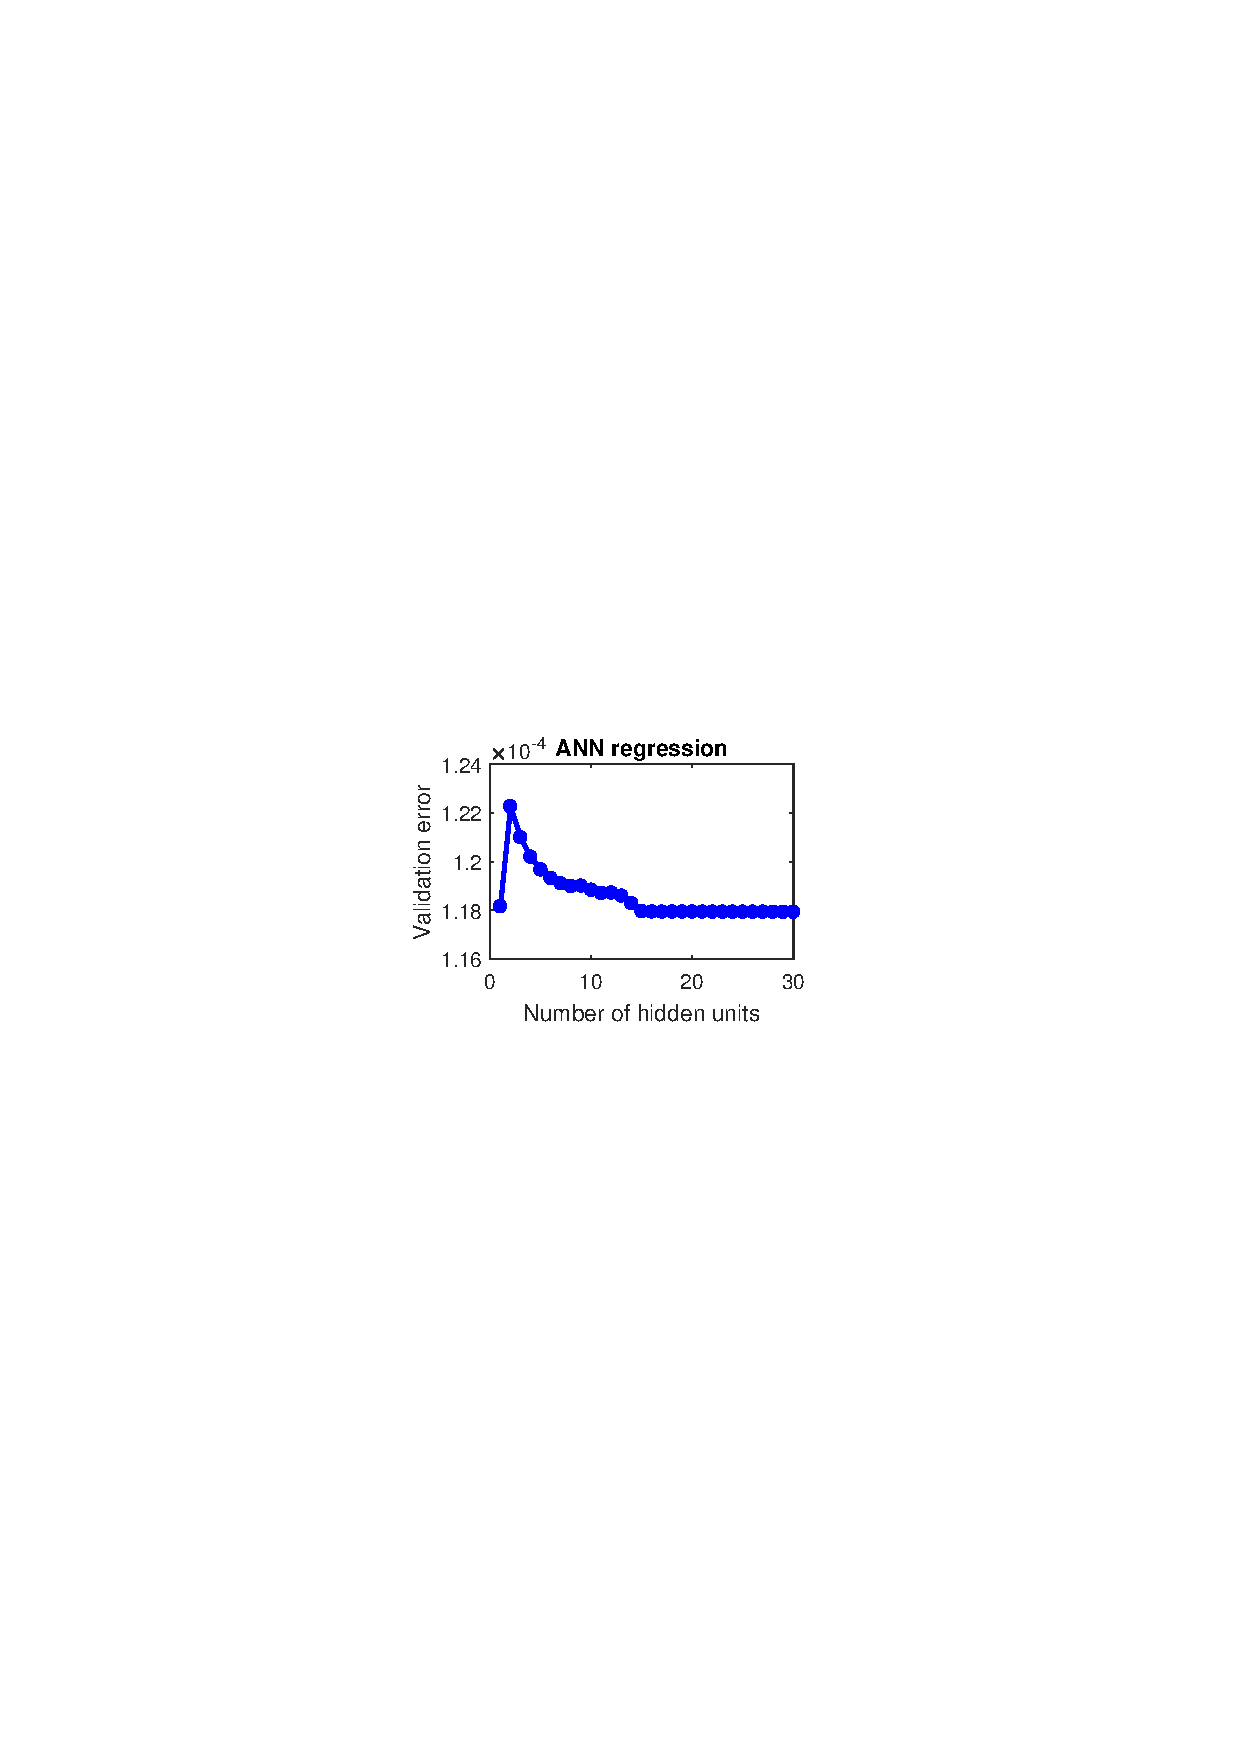
\includegraphics[width=0.40\textwidth]{fig/regression/ANN_reg_validation_error_nmax_30.pdf}
    \caption{Validation error as a function of number of hidden nodes. The minimum occurs at $H=30$.}
    \label{fig:ANN_reg_validation_error_nmax_30}
\end{figure}
\end{multicols}

\textbf{Evaluating the best model:} Overall, ANN regression to predict refraction index \texttt{RI} was a success. In the final test, every prediction was better than predicting the output to be the average of the training data output, seen in fig \ref{fig:ANN_reg_evaluating_best_model_rbk}. We did not perform regularization, but as seen in fig \ref{fig:ANN_reg_evaluating_best_model_line}, the model does not seem to have high bias nor variance, so regularization does not seem necessary.

\begin{multicols}{2}
\begin{figure}[H]
    \centering
    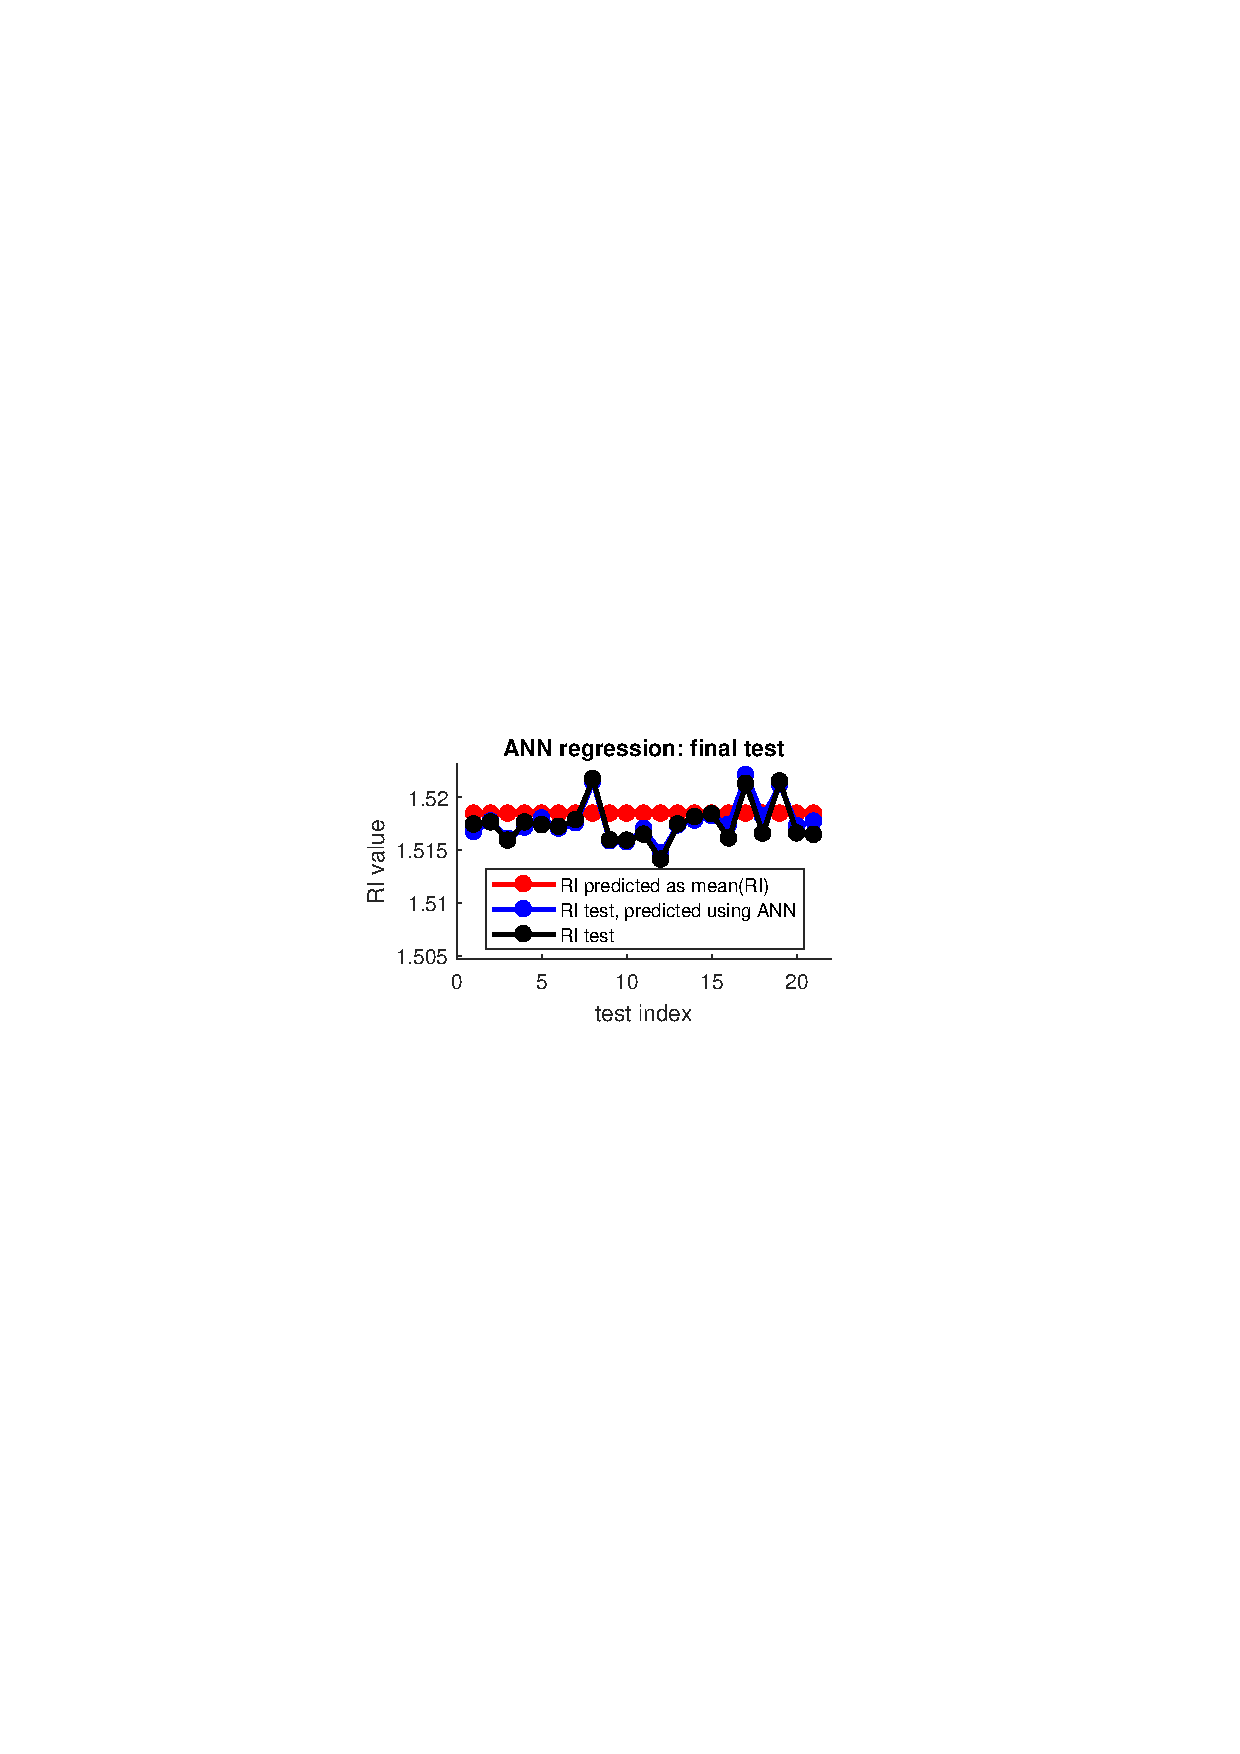
\includegraphics[width=0.50\textwidth]{fig/regression/ANN_reg_evaluating_best_model_rbk.pdf}
    \caption{Comparison between predicted values using simple prediction, ANN prediction ($H=30$), and actual test values.}
    \label{fig:ANN_reg_evaluating_best_model_rbk}
\end{figure}

\begin{figure}[H]
    \centering
    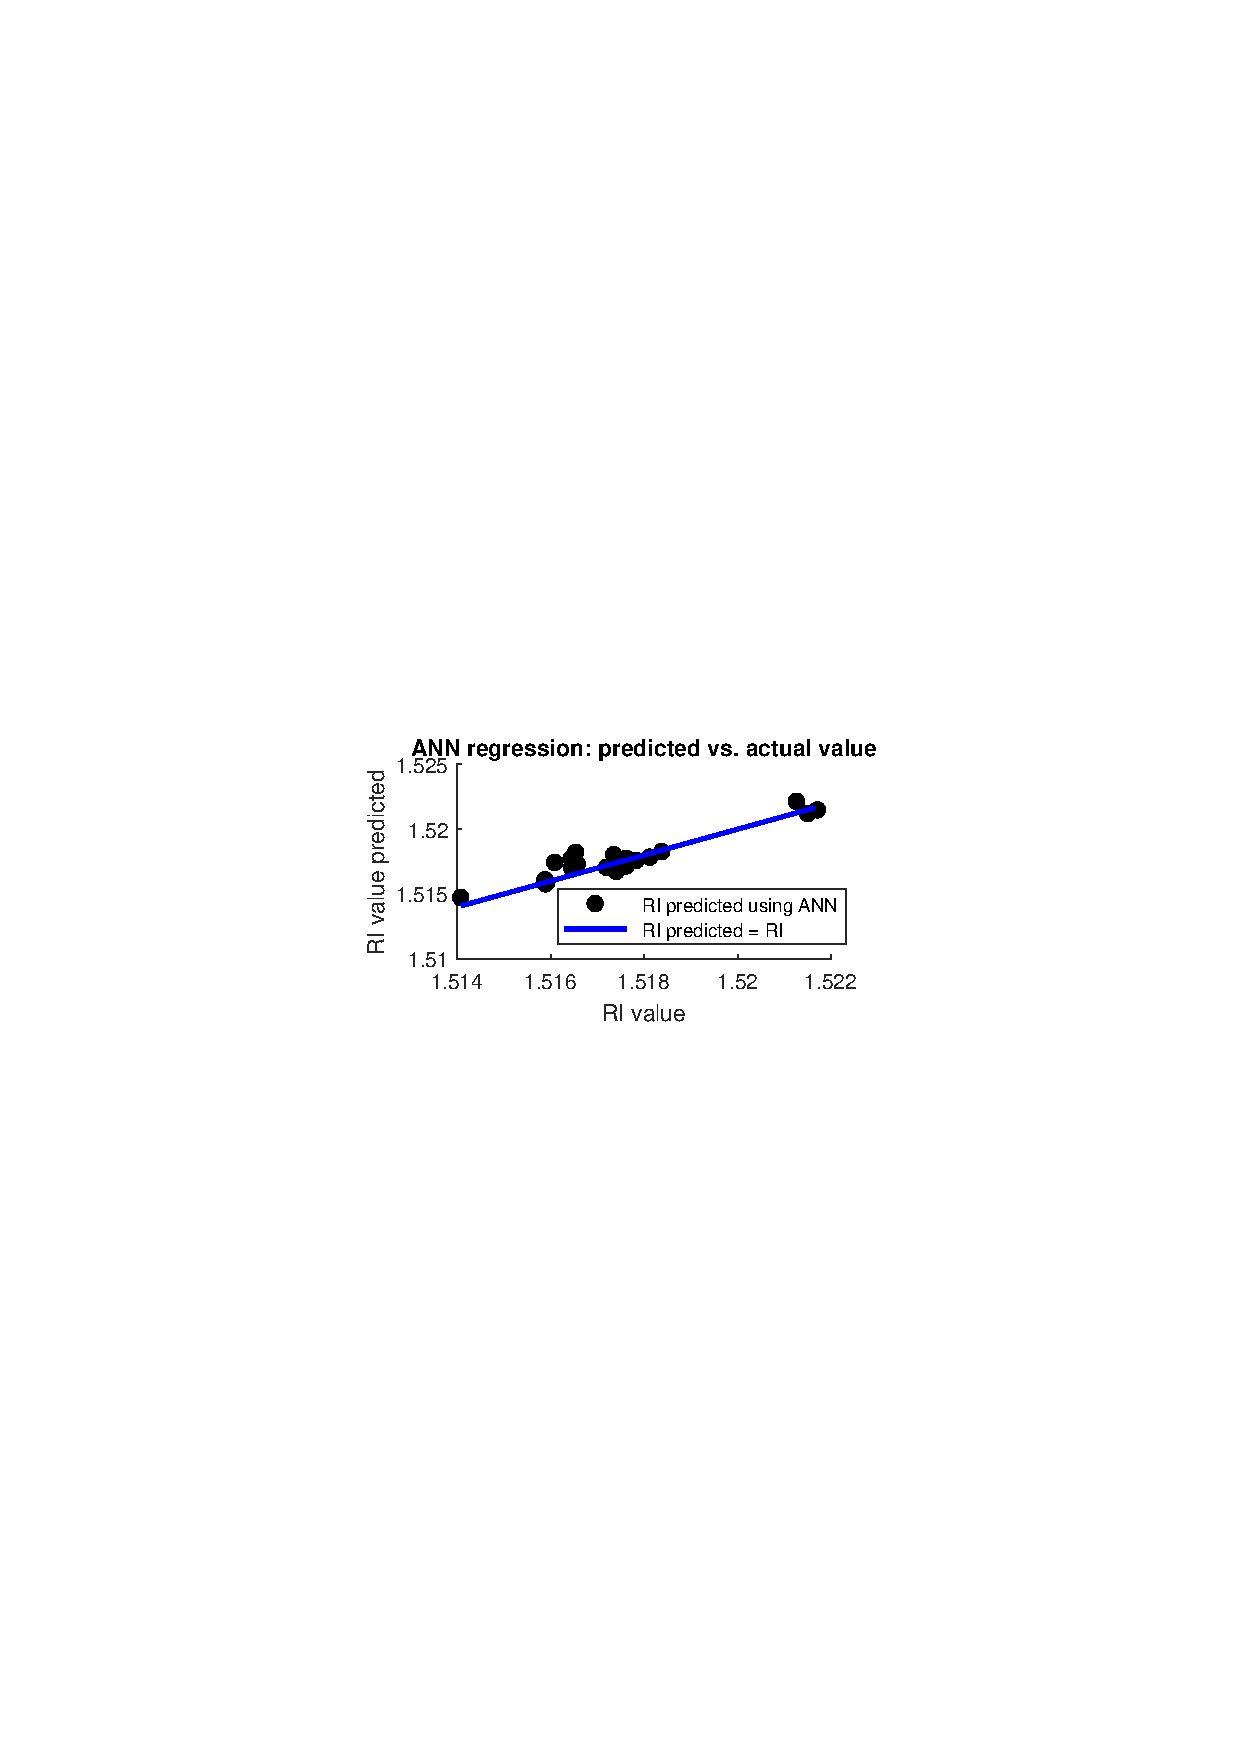
\includegraphics[width=0.50\textwidth]{fig/regression/ANN_reg_evaluating_best_model_line.pdf}
    \caption{Predicted value as a function of actual test observation value.}
    \label{fig:ANN_reg_evaluating_best_model_line}
\end{figure}
\end{multicols}
